
% ----------------------------
% Slide 1: Giới thiệu chung và Mục tiêu kiểm thử
% ----------------------------
\begin{frame}[t]
\frametitle{Giới thiệu chung và Mục tiêu kiểm thử}
\begin{columns}[T]
    \column{0.5\textwidth}
    Trước khi phân tích hiệu năng, các thử nghiệm chức năng được thực hiện nhằm xác nhận từng thành phần của hệ thống hoạt động đúng như thiết kế.
    \begin{itemize}
        \item Xác minh quy trình khởi tạo, kết nối, và truyền dữ liệu.
        \item Đánh giá hiệu quả thuật toán phát hiện té ngã.
        \item Kiểm chứng tính ổn định của các kênh cảnh báo.
        \item Tổng hợp và phân tích log, hình ảnh thực tế.
    \end{itemize}
\end{columns}
\end{frame}

% ----------------------------
% Slide 2: Khởi tạo hệ thống & Module cảm biến đeo
% ----------------------------
\begin{frame}[t,fragile]
\frametitle{Khởi tạo hệ thống \& Module cảm biến đeo}
\begin{columns}[T]
    \column{0.5\textwidth}
    \textbf{1. Khởi tạo hệ thống}
    \begin{itemize}
        \item Các module SIM4G-GPS, Wi-Fi và các tác vụ chính hoạt động bình thường.
        \item Nền tảng phần mềm và phần cứng tích hợp ổn định.
    \end{itemize}
    \vspace{0.2cm}
    \textbf{2. Module 4G/GPS}
    \begin{itemize}
        \item Giao tiếp AT command: OK.
        \item Kết nối 4G, thu nhận GPS ổn định (\texttt{CSQ: 31,99}).
        \item Tọa độ GPS hợp lệ sau vài giây.
    \end{itemize}

    \column{0.5\textwidth}
    \textbf{Log tiêu biểu:}
    \begin{minted}[fontsize=\scriptsize,breaklines]{text}
I (5329) SIM_4G: Received: +CSQ: 31,99
OK
I (10011) APP_MAIN: System initialization complete.
I (10021) APP_MAIN: Application started successfully
I (34349) SIM_4G: Received: +QGPSLOC: 10.88862,106.77975
OK
    \end{minted}
\end{columns}
\end{frame}

% ----------------------------
% Slide 3: Kết nối MQTT và truyền dữ liệu
% ----------------------------
\begin{frame}[t,fragile]
\frametitle{Kết nối MQTT và truyền dữ liệu}
\begin{columns}[T]
    \column{0.5\textwidth}
    \begin{itemize}
        \item ESP32 kết nối broker MQTT và gửi bản tin định kỳ.
        \item Nội dung: định danh thiết bị, trạng thái té ngã, dữ liệu GPS.
        \item Dashboard hiển thị dữ liệu theo thời gian thực.
    \end{itemize}
    \vspace{0.2cm}
    \textbf{Log MQTT:}
    \begin{minted}[fontsize=\scriptsize,breaklines]{text}
I (19961) USER_MQTT: MQTT_EVENT_CONNECTED
I (39991) JSON_WRAPPER: Created status payload:
{"device_id":"ESP32_DEV_76E48B","fall_detected":false}
    \end{minted}

    \column{0.5\textwidth}
    \centering
    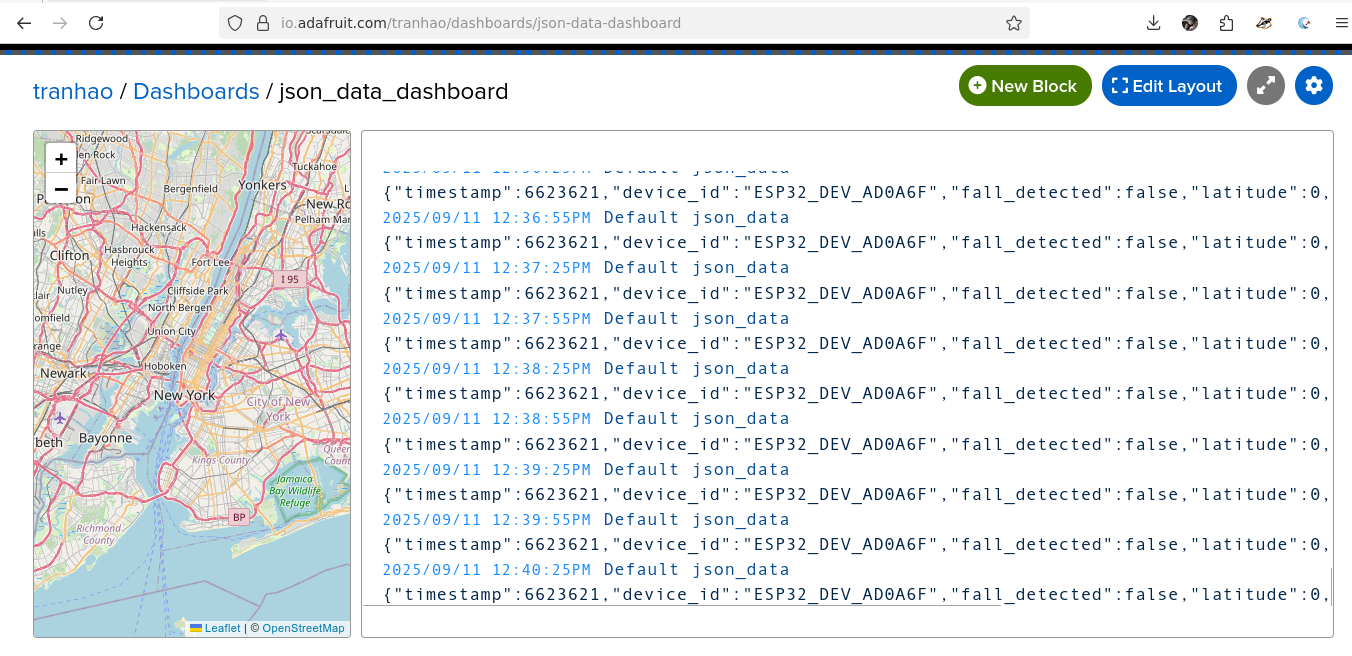
\includegraphics[width=\linewidth]{images/json_data_dashboard.png}
    \captionof{figure}{Dashboard hiển thị bản tin MQTT.}
\end{columns}
\end{frame}

% ----------------------------
% Slide 4: Phát hiện té ngã và cảnh báo
% ----------------------------
\begin{frame}[t,fragile]
\frametitle{Phát hiện té ngã và cảnh báo}
\begin{columns}[T]
    \column{0.5\textwidth}
    \begin{itemize}
        \item Thuật toán kích hoạt khi chuỗi trạng thái \texttt{LOW\_G} $\to$ \texttt{HIGH\_G}.
        \item Cảnh báo đa kênh:
        \begin{itemize}
            \item Gửi SMS/MQTT kèm thông tin định vị.
            \item Kích hoạt buzzer và LED cục bộ.
            \item Gửi thông báo Telegram.
        \end{itemize}
    \end{itemize}
    \vspace{0.2cm}
    \textbf{Log phát hiện té ngã:}
    \begin{minted}[fontsize=\scriptsize,breaklines]{text}
E (159131) FALL_LOGIC: FALL DETECTED! Accel: 0.99 g
I (159151) SIM4G_GPS: SMS request queued successfully
I (159191) SIM4G_GPS: MQTT alert published successfully.
I (159221) buzzer: Beeping for 8000 ms
    \end{minted}

    \column{0.5\textwidth}
    \centering
    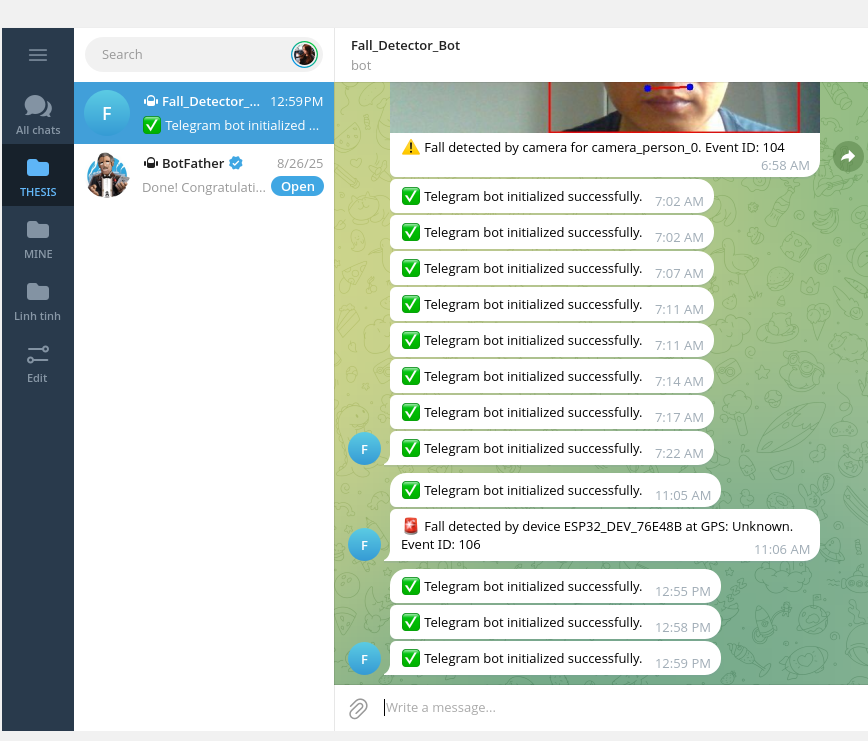
\includegraphics[width=0.9\linewidth]{images/telegram_fall_module1_send.png}
    \captionof{figure}{Thông báo Telegram từ module phần cứng.}
\end{columns}
\end{frame}

% ----------------------------
% Slide 5: Module Camera và xử lý hình ảnh
% ----------------------------
\begin{frame}[t]
\frametitle{Module Camera và xử lý hình ảnh}
\begin{columns}[T]
    \column{0.5\textwidth}
    \textbf{1. ESP32-CAM}
    \begin{itemize}
        \item Kết nối Wi-Fi ổn định.
        \item Phát luồng video HTTP 3.5–5 FPS.
    \end{itemize}
    \textbf{2. Python Module}
    \begin{itemize}
        \item Nhận video, TensorFlow Lite phát hiện người & vẽ skeleton.
        \item Xử lý thời gian thực (3–5 FPS).
    \end{itemize}

    \column{0.5\textwidth}
    \centering
    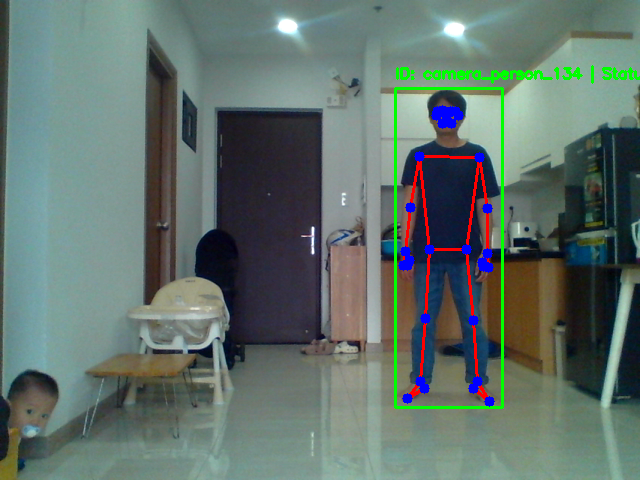
\includegraphics[width=\linewidth]{images/fall_detection_screen_shoot.png}
    \captionof{figure}{Phát hiện người & skeleton từ Python module.}
\end{columns}
\end{frame}

% ----------------------------
% Slide 6: Dữ liệu cảm biến MPU6050
% ----------------------------
\begin{frame}[t]
\frametitle{Dữ liệu cảm biến MPU6050}
\begin{columns}[T]
    \column{0.5\textwidth}
    \begin{table}[h!]
        \caption{So sánh đặc trưng khi té ngã và bình thường.}
        \centering
        \footnotesize
        \begin{tabularx}{\linewidth}{|l|X|X|}
            \hline
            Thông số & Bình thường & Té ngã \\
            \hline
            Độ lớn Gyro (Mag) & 1–2 dps & 100–400 dps \\
            \hline
            Độ lớn Accel (Mag) & 0.95–0.97 g & 0.7–2.0 g \\
            \hline
        \end{tabularx}
    \end{table}
    \vspace{0.2cm}
    \begin{itemize}
        \item Bình thường: \texttt{Accel\_Mag} gần 1\,g, \texttt{Gyro\_Mag} dao động nhỏ.
        \item Té ngã: hai thông số biến thiên mạnh, tạo đỉnh đột biến.
        \item Hậu té: \texttt{Accel\_Mag} trở về gần 1\,g, \texttt{Gyro\_Mag} giảm nhanh.
    \end{itemize}

    \column{0.5\textwidth}
    \centering
    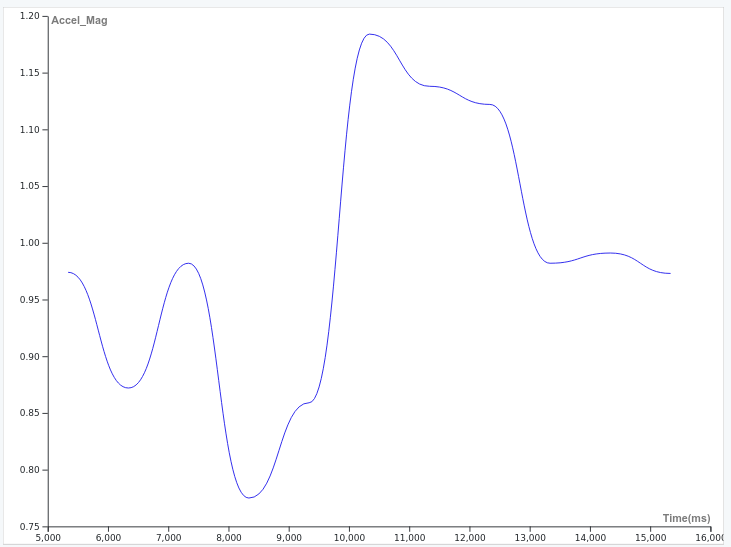
\includegraphics[width=\linewidth]{images/accel_time.png}
    \captionof{figure}{Biến thiên độ lớn gia tốc (Accel\_Mag).}
\end{columns}
\end{frame}

% ----------------------------
% Slide 7: Thử nghiệm GPS và Asterisk AMI
% ----------------------------
\begin{frame}[t]
\frametitle{Thử nghiệm GPS và Asterisk AMI}
\begin{columns}[T]
    \column{0.5\textwidth}
    \textbf{1. GPS}
    \begin{itemize}
        \item Vị trí chính xác: \texttt{10.88862, 106.77975}.
        \item Fix Mode 3, 7 vệ tinh, sai số thấp.
    \end{itemize}
    \textbf{2. Gọi/Nhắn tin (Asterisk AMI)}
    \begin{itemize}
        \item SMS gửi đến \texttt{6001, 6002} thành công.
        \item Gọi điện: lỗi ngoại lệ không ảnh hưởng cơ chế cảnh báo.
    \end{itemize}

    \column{0.5\textwidth}
    \centering
    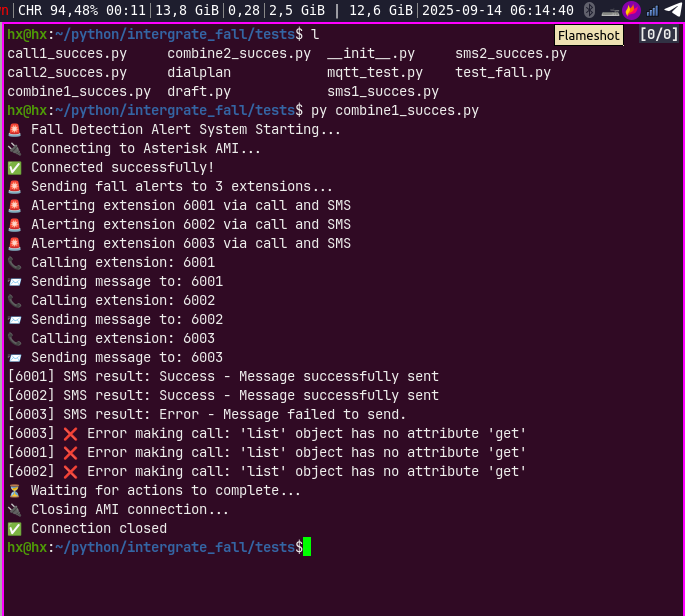
\includegraphics[width=\linewidth]{images/ast_call_sms_test.png}
    \captionof{figure}{Log thử nghiệm Asterisk AMI.}
\end{columns}
\end{frame}

% ----------------------------
% Slide 8: Kênh cảnh báo Telegram
% ----------------------------
\begin{frame}[t]
\frametitle{Kênh cảnh báo Telegram}
\begin{columns}[T]
    \column{0.5\textwidth}
    \begin{itemize}
        \item \textbf{Cảnh báo phần cứng:} ESP32 gửi MQTT, trung tâm chuyển tiếp Telegram.
        \item \textbf{Cảnh báo xử lý hình ảnh:} Python module nhận diện té ngã, gửi trực tiếp Telegram kèm ảnh.
    \end{itemize}

    \column{0.5\textwidth}
    \centering
    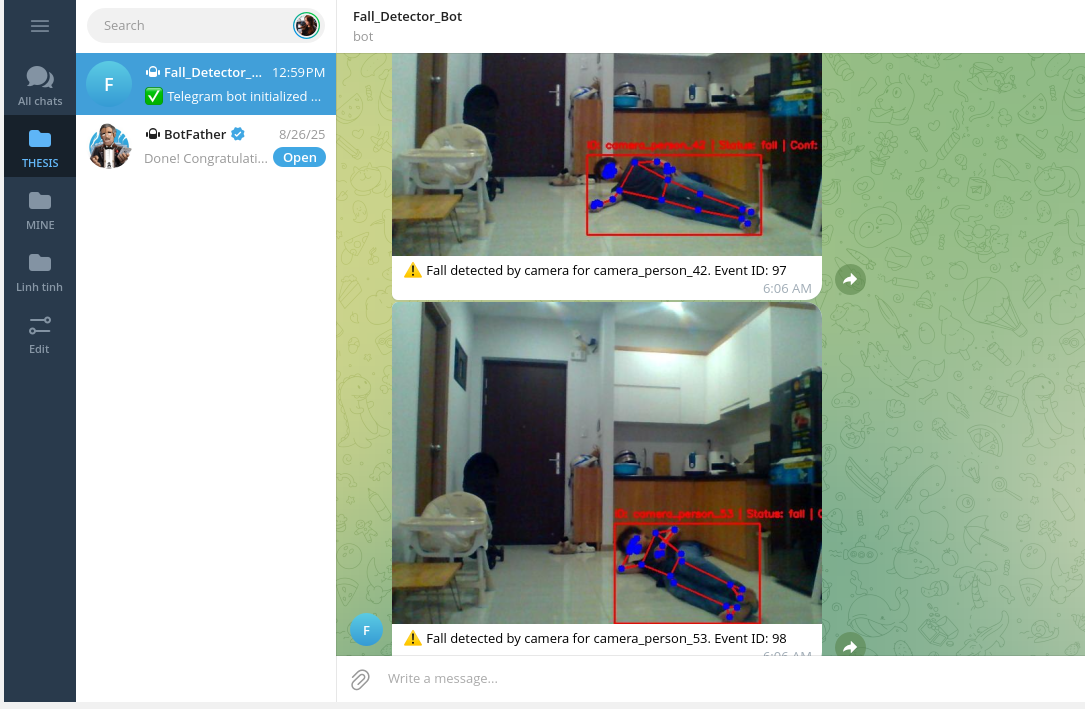
\includegraphics[width=0.9\linewidth]{images/telegram_python_fall_send.png}
    \captionof{figure}{Thông báo từ module Python.}
    \vspace{0.2cm}
    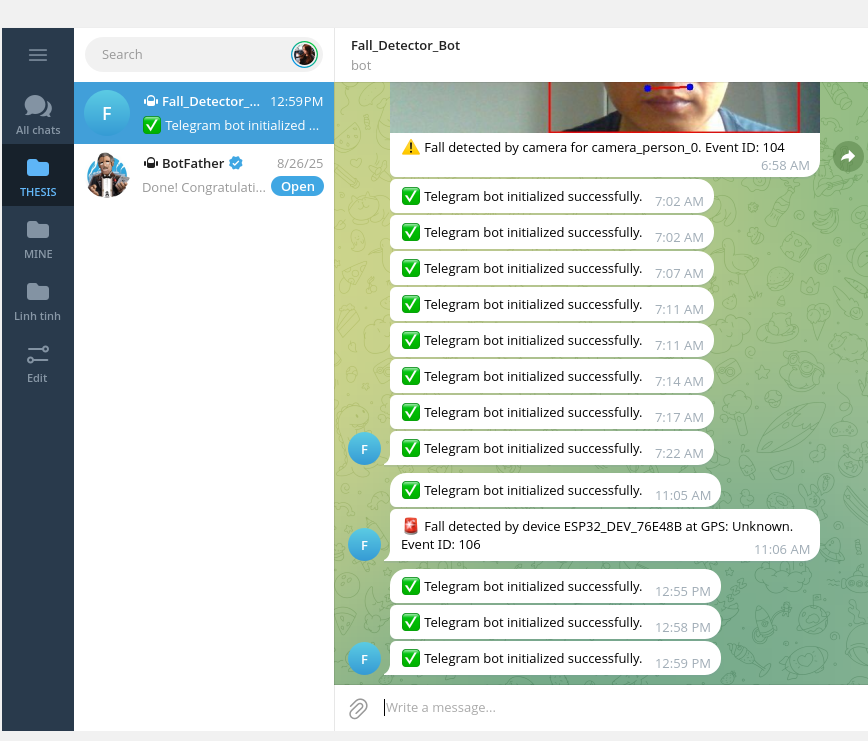
\includegraphics[width=0.9\linewidth]{images/telegram_fall_module1_send.png}
    \captionof{figure}{Thông báo từ module cảm biến đeo.}
\end{columns}
\end{frame}
